\chapter{Proof Sketch}
\label{sec:proof}

Certification of our loop pipelining algorithm naturally requires a certification of each of our primitives.
In addition, we need to ensure that every time a primitive needs to be applied, the conditions
under which the primitive can be applied are maintained. We discuss both aspects below.

\section{Correctness of Primitives}
We must prove that applying a particular primitive is correct, {\em i.e.},
maintaining a certain invariant. This is proven without
considering how it is applied in the context of a pipeline
synthesis algorithm. We give an outline of the proof to justify that the primitives are correct.

{\bf $\phi$-elimination primitive:} We prove that the execution
  of a $\phi$-construct is the same as executing the corresponding
  assignment statements. Note that this is not trivial since
  given a microstep in a scheduling step containing the
  $\phi$-construct, the algorithm has to use static analysis
  to deduce the previous scheduling step.

{\bf Shadow register primitive:} We prove that adding
  a shadow register microstep $x\_reg = x$ does not change the
  value of any variable except the shadow variable. Also, we
  prove that now since value of $x\_reg$ would be equal to value
  of $x$, executing a statement which reads $x$ has the same
  effect on the state as executing a statement which reads
  $x\_reg$ till the next write of $x$. We
  determine the variables read and written in a statement by
  analyzing the execution semantics. Note that $x\_reg$ has to be a new variable which
  is neither written nor read in the given statements.

{\bf Interchange primitive:} We prove that we can interchange two scheduling steps which do not have
  read-write conflict. Given an initial state, the state after
  executing scheduling steps $m$ and $n$ is the same as the state after
  executing $n$ then $m$ if $m$ and $n$ have no read-write
  conflict. Suppose, the state after
  executing $m$ and $n$ is $s_1$ and that after executing $n$ and
  $m$ is $s_2$. We prove that for any variable $x$, its
  value remains same in $s_1$ and $s_2$. After normalizing
  the states, we can prove that $s_1$ is equal to $s_2$, i.e.,
  the states are the same after executing the two scheduling steps in
  a sequence or in an interchanged order. Again, reasoning about read and
  write of statements involves reasoning about execution
  semantics of all types of microsteps present in the
  language which is not trivial.

{\bf Branch primitive:} The proof of the primitive follows from the definition of branch primtive itself as explained in Section 5. This proof would involve semantically analyzing the branch statements and induction on the steps of the CCDFG. 

{\bf Superstep construction primitive:} This primitive is proved
using the interchange primitive and our key invariant described in detail below.

\section{Key Invariant on Correspondence Between Back-edges of Sequential and Pipelined Loops}
 Our key invariant defines a ``correspondence relation''
between the back-edges of the sequential and pipelined CCDFGs.
The relation can be informally paraphrased as
follows~\cite{disha-itp14}.

\begin{quote}
Let $S$ be a sequential loop and $P$ be the pipelined loop
generated from our algorithm. The pipelined loop after superstep construction
consists of
three stages before $S_{preExit}$ as depicted in
Figure~\ref{fig:algo3}(b): prologue $P_{pre}$, full stage
$P_{loop}$, and epilogue $P_{post}$.  Let $s_l$ be any state of $P$
poised to execute $P_{loop}$, and let $k$ be any number such that
the loop of $P$ is not exited in $k$ iterations from $s_l$.
Then executing $P_{pre}$ followed by $k$ iterations of $P_{loop}$ is
equivalent to executing first iteration of $S$, say $S_1$
followed by $(k - 1)$ iterations of $S$ together with a
collection of ``partially completed'' iterations of
$S$.\footnote{The formalization actually characterizes each
  incomplete iteration, \eg, if the pipeline includes $d$
  iterations and successive iterations are introduced in
  consecutive clock cycles, then the $i$-th iteration has $i
  - 1$ incomplete scheduling steps.}
\end{quote}

The partially completed iterations can be determined by the
length of the first iteration in $P_{pre}$ and the pipeline interval.
Suppose the length of the first iteration in $P_{pre}$
is {\tt m} and the pipeline interval is {\tt i}. Note that we
can calculate the value of {\tt m} based on the number of scheduling steps in a CCDFG
and the pipeline interval. The partially completed iterations mean $m$
scheduling steps of $S$ followed by $(m-i)$ scheduling steps of $S$, by
$(m-2i)$ scheduling steps of $S$, etc. while $(m-ni)$ is positive.

In our example, {\tt m} is $2$
and {\tt i} is $1$.  The invariant implies that starting
from the same initial state, executing $P_{pre}$ and {\tt k}
iterations of $P_{loop}$ is the same as executing {\em k}
iterations of $S$, followed by $m = 2$ scheduling steps of
$S$, followed by $ (m - i) = 1$ scheduling steps of $S$.

As is standard with proofs involving invariants, there are
two obligations to prove the correctness, \viz, that it is indeed
an invariant, and that its invariance is sufficient to imply
the desired correctness theorem.  Here we give a sense of
our envisioned proof.

Our invariant is defined specifically to make the proof
sufficiency straightforward.
Equivalence of CCDFG states of $P$ and $S$ follows from the
invariant by noting that the epilogue $P_{post}$ exactly
constitutes the incomplete scheduling steps of $S$ specified
by the invariant
(cf. Figure~\ref{fig:invariant-implies-correctness}).

\begin{figure}[t!]
\begin{center}
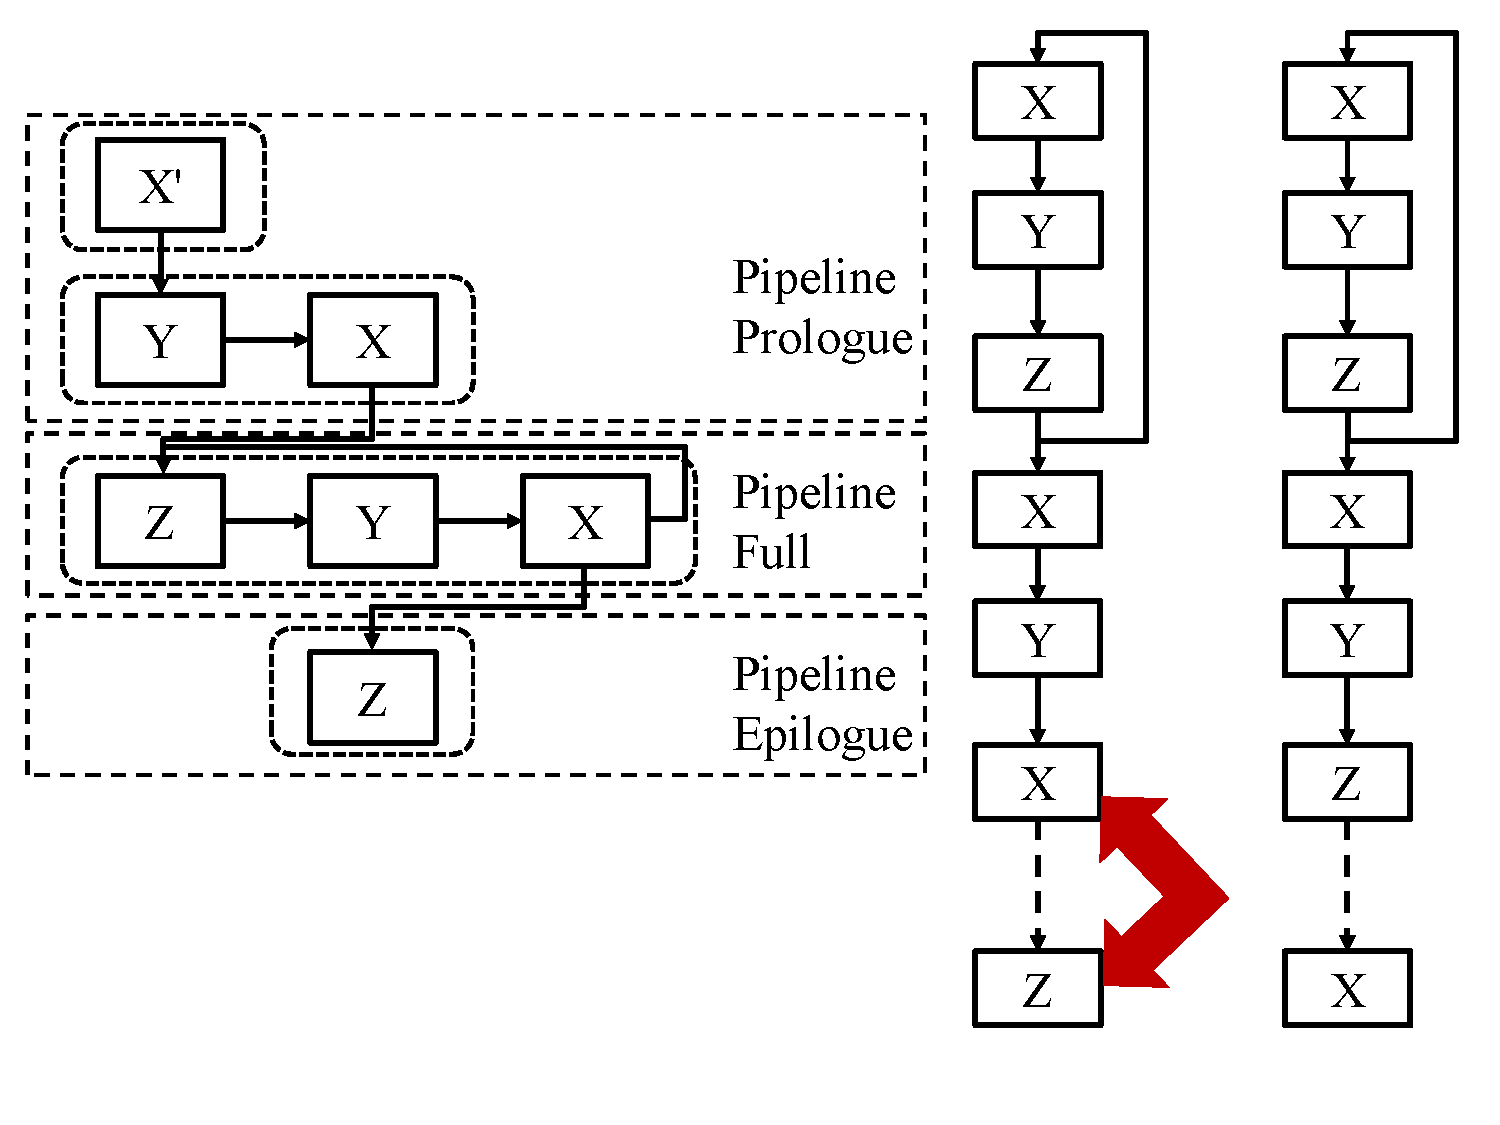
\includegraphics[height=2.2in]{fig-proposal/invariant-implies-correctness}
\end{center}
\caption{Correctness of invariant implies the correctness statement}
\label{fig:invariant-implies-correctness}
\end{figure}

The proof of invariance of this predicate is, of course, the
main ``work horse'' in this exercise.  The proof depends on
our interchange primitive which in turn is based on a fundamental idea for pipelining,
\viz, commutability of
independent instructions.

\begin{quote}
Suppose that the
set of variables written and read by two consecutive
operations $a$ and $b$ is disjoint.  Then executing $a$
followed by $b$ generates the same result as executing $b$
followed by $a$.
\end{quote}

If we view the scheduling steps in
Figure~\ref{fig:high-level-synthesis} as arranged in a
matrix, then the sequential execution proceeds column-wise
along the matrix while the pipelined execution proceeds
row-wise.  Thus the core proof obligation involves the
following two proof requirements.

\begin{enumerate}[--]
\item Our pipelining algorithm correctly combines the
  ``appropriate'' scheduling supersteps which do not have
  read-write hazards.
\item Given that there are no read-write hazards at
  appropriate places, executing scheduling steps row-wise is
  same as executing those scheduling steps column-wise in
  the pipelined CCDFG.  This requires the use of interchange primitive.
\end{enumerate}

\begin{figure}[t!]
\begin{center}
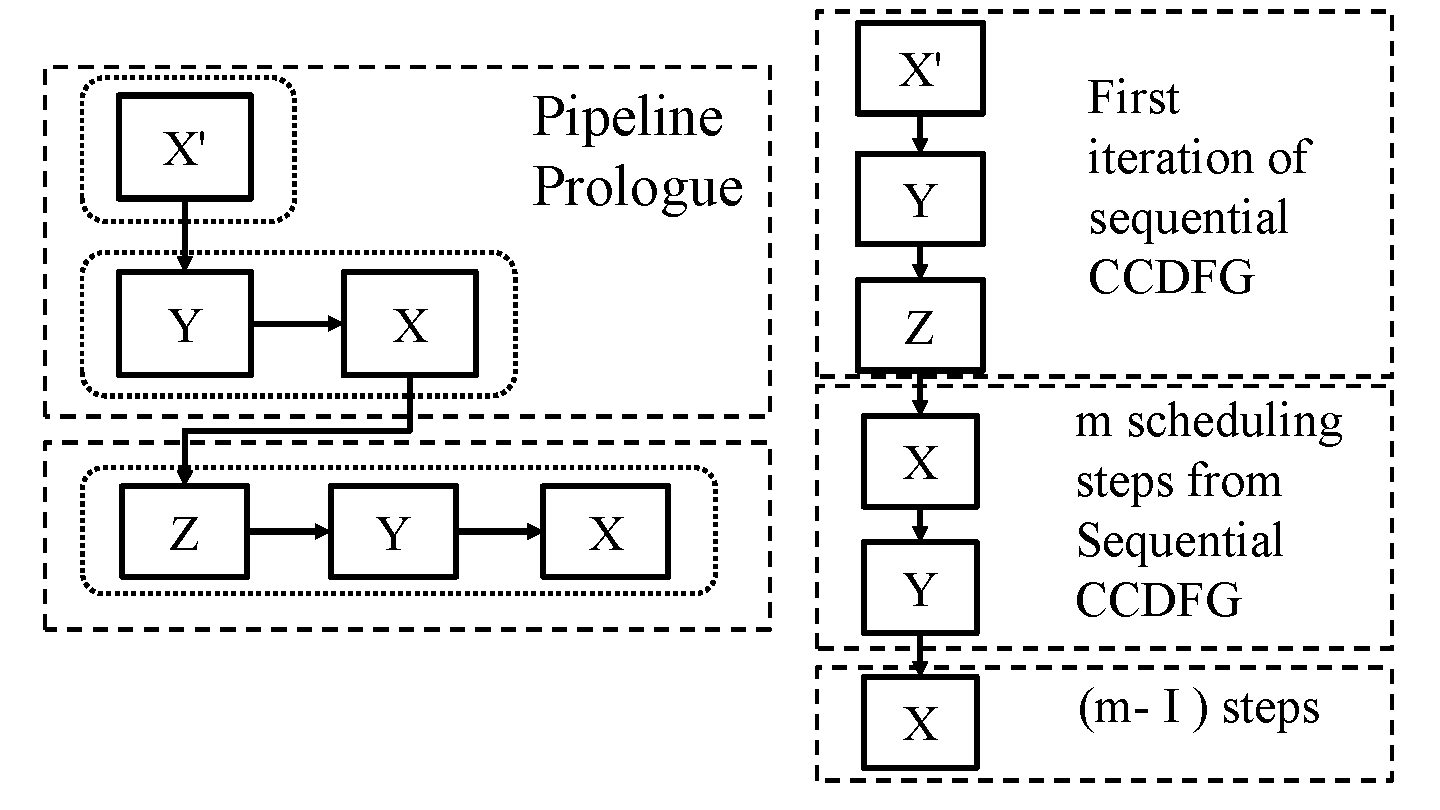
\includegraphics[width=3.5in]{fig-proposal/invariant-base-case}
\end{center}
\caption{Invariant base case where $k = 1$, executing
  pipeline prologue and one pipeline full stage is the same
  as executing $S_{pre}$ followed by a sequence of partially
  completed sequential loop CCDFG.}
\label{fig:invariant-base-case}
\end{figure}

\begin{figure}[t!]
\begin{center}
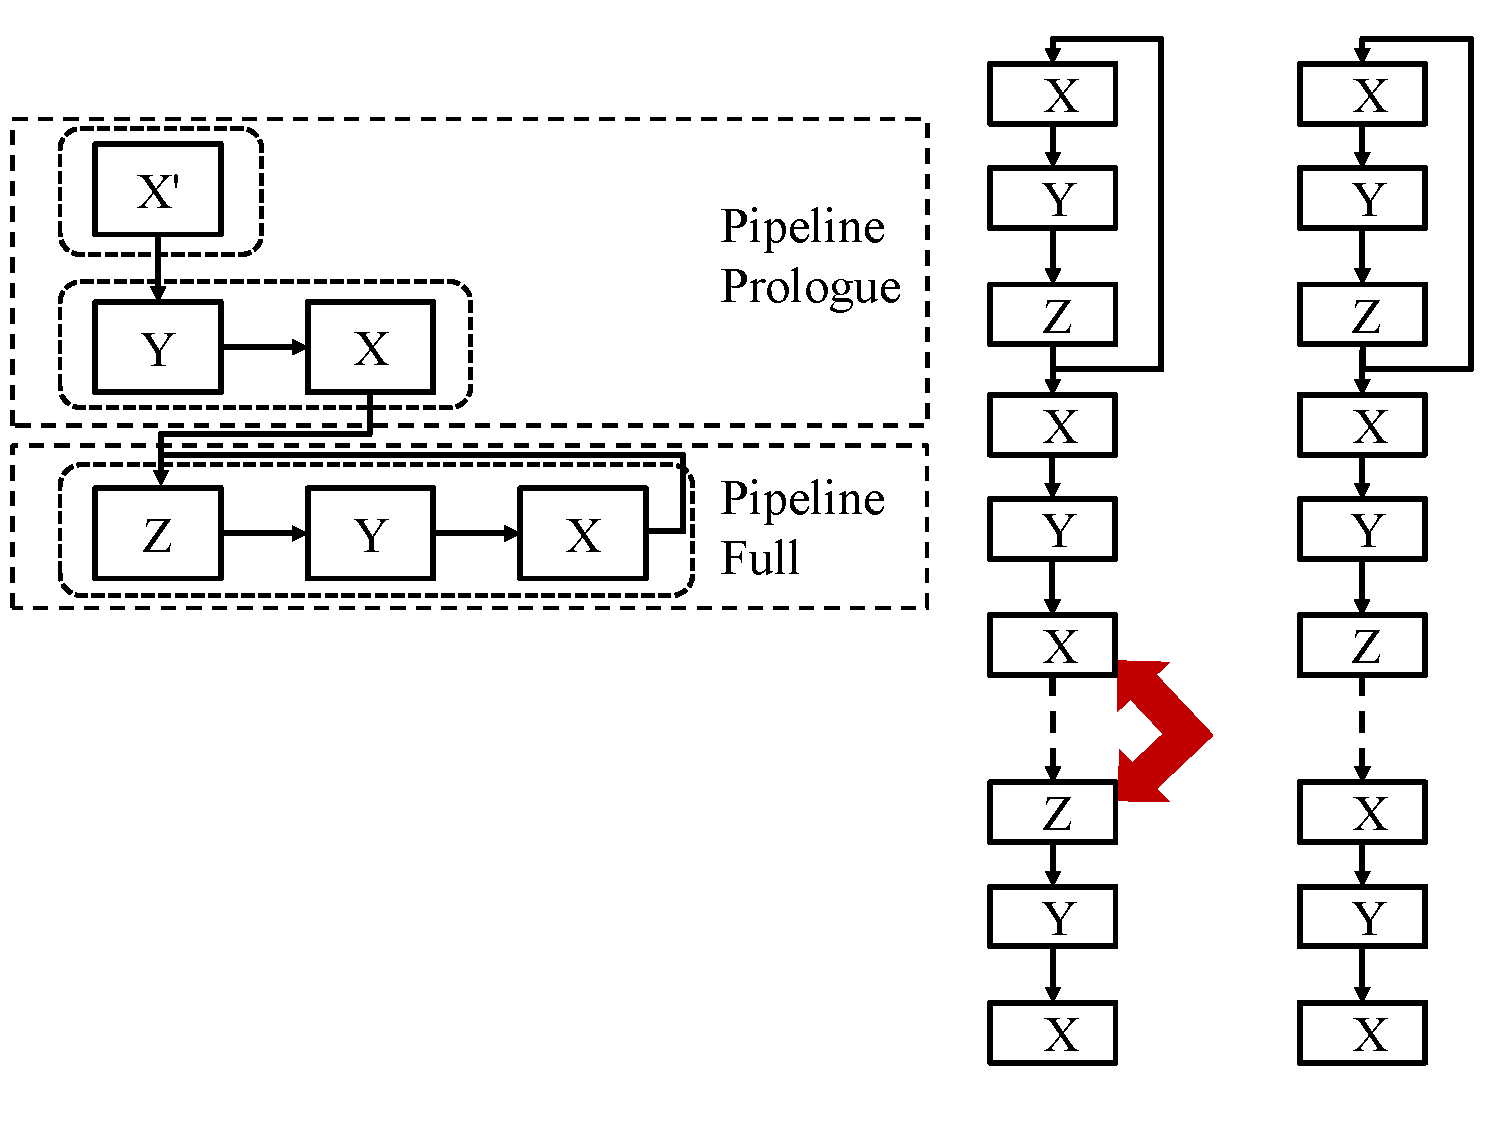
\includegraphics[height=2.2in]{fig-proposal/invariant-inductive-step}
\end{center}
\caption{Assuming that
  invariant is true for $k$ steps, executing one pipeline full
  stage on both sides gives us $(k + 1)$ iterations of
  sequantial loop CCDFG followed by partially completed
  sequences as expected.}
\label{fig:invariant-inductive-step}
\end{figure}

Although these requirements justify that our correspondence
relation is an invariant, they are used somewhat differently
in the base case (when the number of iterations $k$ of the
pipelined loop is $1$) and inductive step (assume the
invariant holds for $k$ iterations of the pipeline and prove
that it holds for $(k+ 1)$ iterations).  Their usage is
pictorially shown in Figures~\ref{fig:invariant-base-case}
and~\ref{fig:invariant-inductive-step}.  For
the base case, we commute operations in the loop prologue of
the pipeline (which corresponds to the first iteration after
unrolling) with the loop body, while for the inductive step
we work with two consecutive iterations of the loop.

Our invariant is very different from a typical invariant
used in the verification of pipelined machines (\eg, for
microprocessor pipelines).  We make explicit the
correspondence with the sequential execution.  The key
requirement from a pipeline invariant, \viz, hazard freedom,
is left implicit and arises indirectly as a proof obligation
for invariance of this predicate.  Most microprocessor
pipeline verification work went the other way.  For
instance, Sawada and Hunt's invariant~\cite{sh:pipeline},
expressed through an intermediate structure called MAETT,
``tracks'' the instructions as they pass through different
pipeline stages to ensure that hazards are not introduced.
One difference in our case is that we are not working with a
concrete pipeline with a fixed set of operations but an
algorithm that generates pipelines with an arbitrary
sequence of scheduling steps; a construction like MAETT is
thus not directly applicable.  However, there is a deeper
reason for defining our invariant the way we did.
Suppose we simply unroll the loop in the sequential
design three times, and then use a technique similar to
MAETT to track scheduling steps in this ``unrolled loop
body'' in the pipeline execution.  Unfortunately, this does
not work, because of the back edge.  There is no direct
correlation between this edge and any edge in the sequential
loop.  In fact, it is interesting to observe what its
introduction achieves: completion of one scheduling step in
each of the three partially executed, overlapping loop
iterations.  This suggests that the invariant must
explicitly capture the state of the executions that have
been partially completed during each iteration of the
pipeline ({\em ie}, each traversal of the back edge).


\section{Correctness of Our Algorithm}

The algorithm is essentially built from ground-up using primitives
as shown in Section~\ref{sec:pipelining-algorithm}. 
However, apart from proving correctness of each primitive and our key invariant,
we also need to ensure that the primitive is applied by our
algorithm properly, {\em i.e.}, the environment
assumptions on which the {\bf correctness of primitive}
depends are maintained appropriately by the algorithm at
the point where the primitive is applied. 
The correctness of each primitive discussed above, entails a
so-called ``assume-guarantee'' reasoning: the primitive is
guaranteed to maintain the desired invariant if and only if
it is applied under certain well-formed conditions.  To use
these correctness statements to verify the algorithm, we
must therefore prove that the algorithm applies each
primitive appropriately, maintaining the well-formedness
condition required for the correctness of the primitive.
Note that verifying this requires an inductive proof
relating the states of the CCDFG $C'$ generated after the
application of the transformation with the original CCDFG
$C$.  The induction is on the lengths of execution of $C$
and $C'$.  Note that the induction is non-trivial because
transformations have significant ``global'' effect on a
CCDFG.  These include one or more of the following:

\begin{enumerate}
\item Replacing one microstep of $C$ with more than one
  microsteps in $C'$ ({\em e.g.}, $\phi$-elimination), or
\item Interchanging scheduling steps ({\em e.g.},
  interchange), or
\item Changing the variable being read or written in several
  microsteps ({\em e.g.}, shadow register)
\end{enumerate}
The upshot is that an inductive theorem relating $C$ and
$C'$ must be strong enough to comprehend the global effects.
For instance, an inductive statement showing the
correctness of $\phi$-elimination must account for the fact
that the number of microsteps of $C$ is different from that
of $C'$.  Thus an execution of $C$ for $n$ microsteps must
correspond to an execution of $C'$ for a different number
$m$ of microsteps, where the number $m$ is a function of $n$
and the structures of $C$ and $C'$; the statement of the
correctness of $\phi$-elimination must characterize the
value of $m$ precisely, perhaps defining functions that
statically and symbolically execute $C$ and $C'$, in order
to be provable by induction.  Furthermore the functions so
introduced for static symbolic execution must themselves be
proven correct.

We can take each stage one by one to understand the complexity involved in 
verifying the algorithm as a whole over and above the verification of 
individual primitives. \textbf{Discusss with Sandip Sir, whether these things are worth mentioning and then elaborate}

In the $AddBranches$ stage, which is the first stage of pipelining algorithm, we 
have to create a correspondence between randomly executing a CCDFG with branches 
using basic-block, sub-basic-block and location with executing a CCDFG without 
a conditional and unconditional branch. This is similar to conditional branch primitive, but since 
we have a random run on one side and a steamlined sequential run on the other side, 
there are theorems involved with finding the next step randomly. 

After this step and for all the subsequent steps, we need to show that there are no relevant branches in CCDFG.

The $\phi-to-assign$ stage, we replace one microstep of $C$ with more than one microsteps in $C'$. 
In addition to inductively reasoning about application of a primitive in entire CCDFG, we also have to ensure
that addition of new microsteps does not affect the basic structure of the CCDFG. These well-formed-conditions
need to be maintained at each step to ensure that the primitives can be applied and they are not trivial.

The data propagation stage, the first step involves identifying the appropriate statements that cause conflict 
and applying interchange primitive. The second step involves moving a statement into the previous iteration. 
In a pre, loop and post, it means removing the statement from beginning of loop and adding it to end of loop. 
Also, statement is adding in end of pre and removed 
from post. {\textbf: Note to Disha: take a look again at this, explain induction with help of diagram if required}.  
These stages need to be
repeated for as many variables as are in conflict. 

In $Shadow-register$ stage, we need to reason about read and write of variables across a number of microsteps. 
This step needs to be repeated as well for multiple variables as required. In this case, however, the reasoning is 
very complicated. Since, after executing shadow register once, we can no longer say that the state in CCDFG-state1 
is same as that of CCDFG-state2, only the real variables have same value. {\textbf: Note to Disha:  elaborate}

In the $Superstep-construction$ stage

In the $AddBranches back$ stage

\section{Lessons from Previous False Starts}

Before we came up with our approach of building a pipelining
algorithm using a framework of certified pipelining primitives,
we tried a few other intuitive approaches.
From each false start, we were able to learn something valuable.

In our initial approach we had decided to simplify the problem
by ignoring the back edge and proving the correspondence
between an unrolled loop and the pipeline.
Only after substantially completing this proof and in
attempting to extend it to the pipeline with the back edge
did we realize that the extension does not work. Section~\ref{sec:proof} describes a key
invariant we defined to deal with this problem.

Also, we attempted initially to stick to the previously proposed algorithm
and try to prove that the semantic run of the input is equal to the semantic run
of the output for the complete algorithm. To do that, we need to claim that
the output pipeline does not introduce any data hazards.
Hazard freedom entails showing the
following. ``Suppose a variable $v$ is written by a
scheduling step $S$ and read subsequently by a scheduling
step $S'$ in the sequential CCDFG.  Then in the pipelined
CCDFG, there is no scheduling step $P$ that writes $v$ and
is executed between $S$ and $S'$.''  Originally, we defined
this notion directly for each variable, \viz, with a
function that statically analyzes the CCDFG to identify the
range of scheduling steps between a write and subsequent
read of each variable.  However, this does not
work.  For example, proving this property for variable $x$
may require a similar property to hold for another variable
$y$ (perhaps because $x$ is assigned an expression involving
$y$).  But the range of scheduling steps in which $x$ and
$y$ are read and written are different, and the extension of
the property to all the variables cannot be easily specified
by an invariant for any specific scheduling step. When we realized
the challenges involved in proving the complete algorithm,
it led us to propose our framework of pipelining primitives.
Also, our current approach succinctly captures an ``on-track property'',
\viz, that the
state after $k$ pipeline iterations is equivalent to partial
execution of a certain number of iterations in the
sequential CCDFG (in addition to completion of $k'$
iterations) which avoids this problem and can indeed be
specified as an invariant.

